\documentclass[a4paper, 12pt,twoside]{book}

% set the paper size and the margins
\usepackage[top = 2cm, bottom = 2cm, left = 2cm, right = 4cm ]{geometry}
\usepackage[showboxes]{textpos}
\setlength{\TPHorizModule}{10mm}
\setlength{\TPVertModule}{\TPHorizModule}
\TPMargin{2mm}
% set the header and the footnote
\usepackage{fancyhdr}
% Supress the hyphenation
\hyphenation{thatshouldnot} 
% for table and equations
\usepackage{tablefootnote}
\usepackage{amsmath,amsfonts,amsthm}
\usepackage{multirow}
\usepackage{hhline}
% make a wide hat for the least-squares regression line
 \usepackage{scalerel,stackengine}
\stackMath
\newcommand\reallywidehat[1]{%
\savestack{\tmpbox}{\stretchto{%
  \scaleto{%
    \scalerel*[\widthof{\ensuremath{#1}}]{\kern-.6pt\bigwedge\kern-.6pt}%
    {\rule[-\textheight/2]{1ex}{\textheight}}%WIDTH-LIMITED BIG WEDGE
  }{\textheight}% 
}{0.5ex}}%
\stackon[1pt]{#1}{\tmpbox}%
}
\usepackage[shortlabels]{enumitem}

% knitr packages
\usepackage[]{graphicx}
\usepackage[]{color}
%% maxwidth is the original width if it is less than linewidth
%% otherwise use linewidth (to make sure the graphics do not exceed the margin)
\makeatletter
\def\maxwidth{ %
  \ifdim\Gin@nat@width>\linewidth
    \linewidth
  \else
    \Gin@nat@width
  \fi
}
\makeatother

\definecolor{fgcolor}{rgb}{0.345, 0.345, 0.345}
\newcommand{\hlnum}[1]{\textcolor[rgb]{0.686,0.059,0.569}{#1}}%
\newcommand{\hlstr}[1]{\textcolor[rgb]{0.192,0.494,0.8}{#1}}%
\newcommand{\hlcom}[1]{\textcolor[rgb]{0.678,0.584,0.686}{\textit{#1}}}%
\newcommand{\hlopt}[1]{\textcolor[rgb]{0,0,0}{#1}}%
\newcommand{\hlstd}[1]{\textcolor[rgb]{0.345,0.345,0.345}{#1}}%
\newcommand{\hlkwa}[1]{\textcolor[rgb]{0.161,0.373,0.58}{\textbf{#1}}}%
\newcommand{\hlkwb}[1]{\textcolor[rgb]{0.69,0.353,0.396}{#1}}%
\newcommand{\hlkwc}[1]{\textcolor[rgb]{0.333,0.667,0.333}{#1}}%
\newcommand{\hlkwd}[1]{\textcolor[rgb]{0.737,0.353,0.396}{\textbf{#1}}}%
\let\hlipl\hlkwb
\usepackage{framed}
\makeatletter
\newenvironment{kframe}{%
 \def\at@end@of@kframe{}%
 \ifinner\ifhmode%
  \def\at@end@of@kframe{\end{minipage}}%
  \begin{minipage}{\columnwidth}%
 \fi\fi%
 \def\FrameCommand##1{\hskip\@totalleftmargin \hskip-\fboxsep
 \colorbox{shadecolor}{##1}\hskip-\fboxsep
     % There is no \\@totalrightmargin, so:
     \hskip-\linewidth \hskip-\@totalleftmargin \hskip\columnwidth}%
 \MakeFramed {\advance\hsize-\width
   \@totalleftmargin\z@ \linewidth\hsize
   \@setminipage}}%
 {\par\unskip\endMakeFramed%
 \at@end@of@kframe}
\makeatother


\definecolor{shadecolor}{rgb}{.97, .97, .97}
\definecolor{messagecolor}{rgb}{0, 0, 0}
\definecolor{warningcolor}{rgb}{1, 0, 1}
\definecolor{errorcolor}{rgb}{1, 0, 0}
\newenvironment{knitrout}{}{} % an empty environment to be redefined in TeX

\usepackage{alltt}


% packages will be used by the 'kable' package
\usepackage{booktabs}
\usepackage{longtable}
\usepackage{array}
\usepackage{multirow}
\usepackage[table]{xcolor}
\usepackage{wrapfig}
\usepackage{float}
\usepackage{colortbl} 
\usepackage{pdflscape}
\usepackage{tabu}
\usepackage{threeparttable}
\usepackage{threeparttablex}
\usepackage[normalem]{ulem}
\usepackage{makecell}
\usepackage{xcolor}
\IfFileExists{upquote.sty}{\usepackage{upquote}}{}

% define a color for highlight
\definecolor{asparagus}{rgb}{0.53, 0.66, 0.42}
\definecolor{babypink}{rgb}{0.96, 0.76, 0.76}
\definecolor{champagne}{rgb}{0.97, 0.91, 0.81}
\definecolor{forestgreen}{rgb}{0.13, 0.55, 0.13}
\definecolor{dollarbill}{rgb}{0.52, 0.73, 0.4}

\usepackage{tcolorbox}

\tcbset{width=0.9\textwidth,boxrule=0pt,colback=champagne,arc=0pt,
auto outer arc,left=0pt,right=0p}

\usepackage{hhline}

\usepackage{amsmath}

\setlength{\parindent}{0.5cm} 

\usepackage{siunitx}

%Chinese yen
\usepackage{stackengine}
\newcommand{\textyen}{\stackengine{-6pt}{=}{\large{\text{Y}}}{O}{c}{F}{T}{S}}

\setlength{\parindent}{0cm}

\begin{document}

%Deal with the headers of each chapter
\pagestyle{fancy}
\fancyhf{}
\renewcommand{\chaptermark}[1]{ \markboth{#1}{} }
\fancyhead[CE,CO]{\leftmark}
\fancyfoot[LE,RO]{\thepage}

\chapter{Hypothesis Test}
A report says the average yearly income of Chinese people is 74,318\textyen, but you suspect the average income is less than reported. Is your suspicion correct? In this chapter, we will learn how to solve this problem through \textbf{hypothesis test}.
\newpage

\section{Basics of Hypothesis Test}

  In order to test whether a given coin is fair or not, it is tossed 100 times, and resulted in 45 heads. Does this provides convincing evidence that this coin is not fair?\vspace{0.3cm}

\begin{itemize}
\item \textbf{Hypotheses}\vspace{0.3cm}

In the above setting, we have two contending \textbf{hypotheses} about the parameter $p$ , where $p$ is the probability of getting a head when this coin is tossed. One hypothesis is $\displaystyle{p=\frac{1}{2}}$, which means the coin is fair. The other one is $\displaystyle{p \ne \frac{1}{2}}$, which means the coin is not fair. The firs hypothesis is called \textbf{null hypothesis}, denoted as $\textbf{H}_0$, and the second one is called \textbf{alternative hypothesis}, denoted as $\textbf{H}_a$. They are written as 
$$\textbf{H}_0:\quad p=\frac{1}{2}$$
$$\textbf{H}_a:\quad p\ne\frac{1}{2}$$
\colorbox{babypink}{\parbox{0.9\textwidth}{
\textbf{Remark:}
\begin{itemize}
\item Usually, the $\textbf{H}_a$ is the hypothesis we want to seek evidence for.
 \item The hypotheses are about parameters. 
You can not set statements like $\reallywidehat{p} = \frac{1}{2}$, $\bar{x} = 0.6$ as hypotheses.
 \end{itemize}
}}
\vspace{0.3cm}

 The \textbf{hypothesis test} is the procedure to make decisions between the two hypotheses.\vspace{0.3cm}

In the above case, if $\textbf{H}_a$ is true, it can either be $p < \frac{1}{2}$ or $p > \frac{1}{2}$. This type of \textit{hypotheses test} is called \textbf{two-sided hypotheses test}.\vspace{0.3cm}

If the hypotheses are set as either of the following

$$\textbf{H}_0:\quad p=\frac{1}{2}, \qquad \textbf{H}_a:\quad p >\frac{1}{2}$$

$$\textbf{H}_0:\quad p=\frac{1}{2}, \qquad \textbf{H}_a:\quad p <\frac{1}{2}$$

the \textit{hypotheses test} is called \textbf{one-sided hypotheses test}.\vspace{0.6cm}

\colorbox{champagne}{\parbox{0.9\textwidth}{
\textbf{Juicy Pineapples}\vspace{0.3cm}

At the Hawaii Pineapple Company, managers are interested in the size of the pineapples grown in the company’s fields. Last year, the mean weight of the pineapples harvested from one large field was 31 ounces. A  different irrigation system was installed in this field after the growing season.  Managers wonder how this change will affect the mean weight of  pineapples grown in the field this year.\vspace{0.3cm}
\begin{enumerate}[(a)]
    \item State appropriate hypotheses for performing a significance test. Be sure to define the parameter of interest.
    \item Is this a \textbf{one-sided} or \textbf{two-sided} hypotheses test?
\end{enumerate}
}}
\newpage





\item \textbf{The reasoning of hypotheses test}\vspace{0.3cm}

Let's use the ``fair coin'' setting and the hypotheses are
$$\textbf{H}_0:\quad p=\frac{1}{2}$$
$$\textbf{H}_a:\quad p\ne\frac{1}{2}$$ 
Among the 100 tosses, 45 are head.\vspace{0.3cm}

How to choose between those two hypotheses? The reasoning is like:   if we assume the \textit{null hypotheses} is true, and we get a sample with the sample proportion $\hat{p}$ far away from $\displaystyle p= \frac{1}{2}$, then we have convincing evidence for $H_a$ and reject $H_0$. \vspace{0.3cm}

\textbf{In the following, $H_0$ is assumed to be true, with $p = 1/2$!!!}\vspace{0.3cm}


How to tell whether $\reallywidehat{p}$ is far away from $p$ or not? We have to resort to the sampling distribution of $\reallywidehat{p}$ when assuming $H_0$ is true. According to what we learned before, if certain conditions are met, $\reallywidehat{p}$ is approximately normally distributed. 
$$\reallywidehat{p} \sim N(\mu_{\reallywidehat{p}}, \sigma_{\reallywidehat{p}}), \qquad \mu_{\reallywidehat{p}} = p, \quad \sigma_{\reallywidehat{p}} = \sqrt{\frac{p(1-p)}{n}}$$     
    \begin{figure}[H]
    \centering
    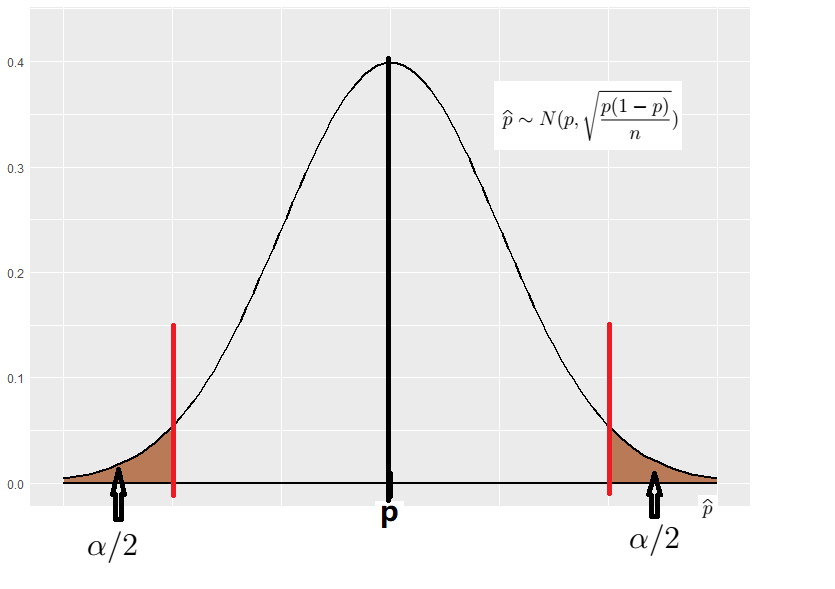
\includegraphics[scale=0.6]{HypothesisTestSamplingDistribution}
    \caption{$\hat{p}$ that is far away from $p$}
    \label{HypothesisTestSamplingDistribution}
    \end{figure}
    


In figure\ref{HypothesisTestSamplingDistribution}, we draw two lines away from $p$. If a $\reallywidehat{p}$ falls to the outside of those two lines, indicated by the shaded areas, we say this $\reallywidehat{p}$ is far away from $p$.\vspace{0.3cm}

However, where to draw those two lines? Referring to figure\ref{HypothesisTestSamplingDistribution}, if the total area of the ``shaded areas'' are given, then the position of the two lines are decided. We call this given total area \textbf{significance level $\mathbf{\alpha}$}. The most frequently used \textit{significance level} is $\mathbf{\alpha} = 0.05$.

\begin{textblock}{3}(15.5, -5)
\textblockcolor{dollarbill}
Set significance level $\mathbf{\alpha} = 0.05$. Is the $\reallywidehat{p}$ far away from $p$ in the case of ``fair coin'' with $$H_0 = 1/2$$ $$H_a \ne 1/2$$
\end{textblock}
\vspace{0.3cm}

In the above \textit{two-sided hypotheses}, when $\reallywidehat{p}$ is either way larger or way smaller than $p$, we say $\reallywidehat{p}$ is far away from $p$ in the direction of $H_a$. Because, either ``way larger'' or ``way smaller'' is in favour of $H_a$.\vspace{0.3cm}

How to define ``far away'' in the case of \textit{one-sided hypotheses test}? Use the ``fair coin'' example, and change the hypotheses into 
    $$\textbf{H}_0:\quad p=\frac{1}{2}$$
$$\textbf{H}_a:\quad p\leq \frac{1}{2}$$ 

Since we have to decide whether  $\reallywidehat{p}$ is far away from $p$ in the direction of $H_a$, we have to draw a borderline to the left side of $p$, as shown in figure\ref{OneSidedHT}.    
     \begin{figure}[H]
     \centering
     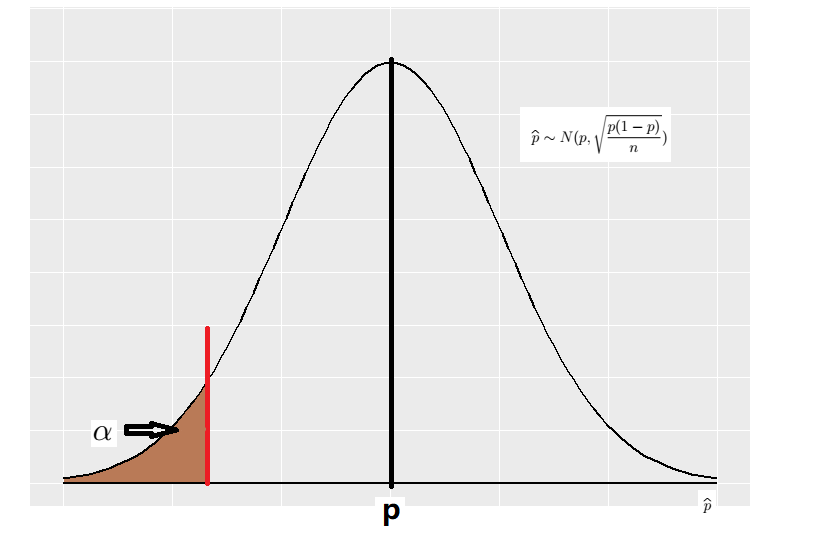
\includegraphics[scale=0.6]{OneSidedHT}
     \caption{One-sided hypotheses test}
     \label{OneSidedHT}
     \end{figure}
Here, the \textit{significance level} $\mathbf{\alpha}$ is the area to the left side of the borderline demarcating whether $\reallywidehat{p}$ is far away from $p$ or not.

\begin{textblock}{3.6}(-3, -4)
\textblockcolor{dollarbill}
Set significance level $\mathbf{\alpha} = 0.05$. Is the $\reallywidehat{p}$ far away from $p$ in the case of ``fair coin'' with $$H_0 = 1/2$$ $$H_a \leq 1/2$$
\end{textblock}
\vspace{0.6cm}

In the case of \textit{one-sided hypotheses test} as
    $$\textbf{H}_0:\quad p=\frac{1}{2}$$
$$\textbf{H}_a:\quad p\leq \frac{1}{2}$$ 
everything is argued similarly.\vspace{0.6cm}

\colorbox{babypink}{\parbox{0.9\textwidth}{
\textbf{Remark:}\vspace{0.3cm}

 \begin{itemize}
     \item \textbf{Significance level $\alpha$ is set before the sample is drawn.} 
     \item \textbf{The hypotheses is set before the sample is drawn.}
     \item \textbf{All the above are based on the assumption that $H_0$ is true.}
 \end{itemize}

}}

\newpage

\item \textbf{The P-value}\vspace{0.3cm}

Still use the ``fair coin'' example, and the hypotheses are
$$\textbf{H}_0:\quad p=0.5$$
$$\textbf{H}_a:\quad p\ne0.5$$ 
The sample proportion $\reallywidehat{p}_0 = 45/100 = 0.45$.\vspace{0.3cm}

Assume $H_0$ is correct.
$$\textbf{P}(|\reallywidehat{p}-0.5| > |\reallywidehat{p}_0-0.5|)= \textbf{P}(\reallywidehat{p}>0.55) + \textbf{P}(\reallywidehat{p}<0.45)$$
     \begin{figure}[H]
     \centering
     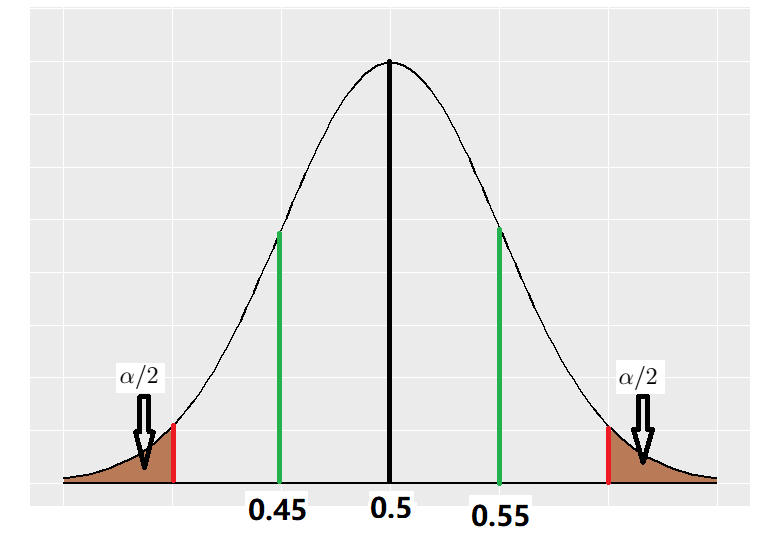
\includegraphics[scale=0.5]{PvalueTwoSided}
     \caption{P-value for two-sided hypotheses test}
     \label{PvalueTwoSided}
     \end{figure}
 
 \begin{textblock}{3.6}(14.5, -6)
\textblockcolor{dollarbill}
Calculate the P-value of the ``fair coin'' example with hypotheses $$\textbf{H}_0:\quad p=0.5$$
$$\textbf{H}_a:\quad p\ne0.5.$$ 
\end{textblock}


Reading figure\ref{PvalueTwoSided}, we know that if
$\textbf{P}(|\reallywidehat{p}-0.5| \geq |\reallywidehat{p}_0-0.5|)\geq \alpha $, then the sample proportion $\reallywidehat{p}_0$ is not far away from $H_0$ in the direction of $H_a$ under the significance level $\alpha$. We fail to reject $H_0$, and don't have convincing evidence for $H_a$. 
 If $\textbf{P}(|\reallywidehat{p}-0.5| \geq |\reallywidehat{p}_0-0.5|)< \alpha$, then the sample  proportion $\reallywidehat{p}_0$ is  far away from $H_0$ in the direction of $H_a$ under the significance level $\alpha$. We reject $H_0$ and have convincing evidence for $H_a$.\vspace{0.3cm}

In the above \textit{two-sided hypotheses test}, $\textbf{P}(|\reallywidehat{p}-0.5| \geq |\reallywidehat{p}_0-0.5|)$ plays an important role in making conclusions. It is called the \textbf{P-value} of the test.\vspace{0.3cm}

$\textbf{P}(|\reallywidehat{p}-0.5| \geq |\reallywidehat{p}_0-0.5|)$ is the probability of getting a $\reallywidehat{p}$ as extreme as or more extreme than the observed $\reallywidehat{p}-0$ in the direction of $H_a$. A more formal definition of \textit{P-value} is given below.\vspace{0.3cm}

\colorbox{babypink}{\parbox{\textwidth}{
\textbf{P-value} is the probability, computed assuming $H_0$ is true, that the statistic(such as $\reallywidehat{p}$ or $\bar{x}$) would be as extreme as or more extreme than the observed value, in the direction of $H_a$.
}}
\vspace{0.3cm}

Sometimes you are asked to interpret the \textit{P-value}. You have to interpret in the context. In the above example we should interpret the \textit{P-value} as ``Assuming the probability of getting a head is 0.5, the probability of tossing 100 times with the relative frequency of heads less than or equal to 0.45, or larger than or equal to 0.55 is `\textit{P-value}' ''.\vspace{0.3cm}


In the ``fair coin'' example, if the hypotheses test is a \textit{one-sided hypotheses test} with hypotheses
$$\textbf{H}_0:\quad p=0.5$$
$$\textbf{H}_a:\quad p\leq 0.5$$ 
The \textit{P-value} is indicated in figure\ref{PvalueOneSide}.
\begin{figure}[H]
\centering
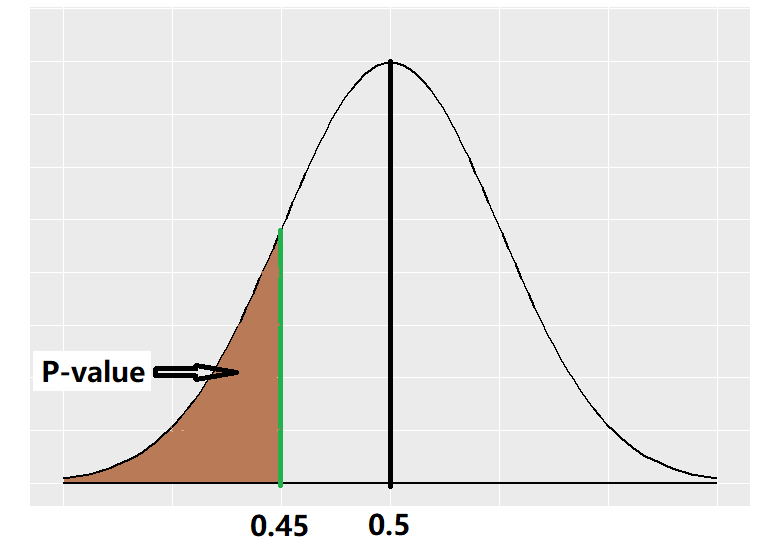
\includegraphics[scale=0.3]{PvalueOneSide}
\caption{P-value for \textit{one-sided hypotheses test}}
\label{PvalueOneSide}
\end{figure}

\begin{textblock}{4}(-3, -5)
\textblockcolor{dollarbill}
Calculate and interpret the P-value of the ``fair coin'' example, with hypotheses $$\textbf{H}_0:\quad p=0.5$$
$$\textbf{H}_a:\quad p\leq 0.5$$ 
\end{textblock}
The characteristics and the definition of \textit{P-value} of \textit{one-sided hypotheses test} is the same as of \textit{two-sided hypotheses test}.\vspace{0.3cm}  

\colorbox{champagne}{\parbox{0.9\textwidth}{
\textbf{Healthy Bones}\vspace{0.3cm}

Calcium is a vital nutrient for healthy bones and teeth. The National Institutes of Health (NIH) recommends a calcium intake of 1300 mg per day for teenagers. The NIH is concerned that teenagers aren’t getting enough calcium. Is this true?\vspace{0.3cm}

Researchers want to perform a test of
$$H_0:\;\mu=1300;\quad H_a:\; \mu< 1300$$
where $\mu$ is the true mean daily calcium intake in the population of teenagers. They ask a random sample of 20 teens to record their food and drink consumption for 1 day. The researchers then compute the calcium intake for each student. Data analysis reveals that $\bar{x} =1198$mg and $s_x = 441$ mg. After checking that conditions were met, researchers performed a significance test and obtained a P-value of 0.1404.\vspace{0.3cm}

\begin{enumerate}[(a)]
    \item Explain what it would mean for the null hypothesis to be true in this setting.
    \item Interpret the P-value in context.
\end{enumerate}
}}



\newpage 
   
\item \textbf{P-value and conclusions} \vspace{0.3cm}

If the \textit{P-value} is smaller than the \textit{significance level} $\alpha$, we say the results of the study are \textbf{statistically significant at level $\alpha$}. In this case, we reject the null hypotheses $H_0$ and conclude that there is convincing evidence for $H_a$. \vspace{0.3cm}

\colorbox{babypink}{\parbox{0.9\textwidth}{
In nutshell, the relation between P-value and conclusions comes down to\vspace{0.3cm}


$\text{P-value} < \alpha \implies \text{reject }H_0 \implies \text{convincing evidence for } H_a$\\
$\text{P-value} > \alpha \implies \text{fail to reject }H_0 \implies \text{no convincing evidence for } H_a$\\
}}
\vspace{0.3cm}

\item \textbf{Test statistic}\vspace{0.3cm}

In the ``fair coin' example, the P-value of the \textit{two-sided hypotheses test} is given by 
  $$\textbf{P}(|\reallywidehat{p}-0.5| > |\reallywidehat{p}_0-0.5|), \qquad\reallywidehat{p}_0= 0.45 $$
  
 If conditions are met,  $\reallywidehat{p}$ follows a normal distribution.
 $$\reallywidehat{p} \sim N(\mu_{\reallywidehat{p}}, \sigma_{\reallywidehat{p}}), \qquad \mu_{\reallywidehat{p}} = p=0.5,\quad\sigma_{\reallywidehat{p}} = \sqrt{\frac{p(1-p)}{n}} = 0.05 $$  

 $$\textbf{P}(|\reallywidehat{p}-0.5| > |\reallywidehat{p}_0-0.5|)= \textbf{P}(|\frac{\reallywidehat{p}-0.5}{\sigma_{\reallywidehat{p}}}| > |\frac{\reallywidehat{p}_0-0.5}{\sigma_{\reallywidehat{p}}}|)=\textbf{P}(|z_{\reallywidehat{p}}|>|z_{\reallywidehat{p}_0}|)$$
 where $z_{\reallywidehat{p}} \sim N(0, 1)$ and $z_{\reallywidehat{p}_0}= -1$. 
 $$\textbf{P-value} = \textbf{P}(|z_{\reallywidehat{p}}|>1)$$
 It is very easy to calculate the P-value by referring to the standard normal distribution.\vspace{0.3cm}
 
 In the above calculation, $z_{\reallywidehat{p}_0}$ is called the \textbf{test statistic}. \vspace{0.3cm}
 
 
\colorbox{babypink}{\parbox{\textwidth}{
The general formula for \textit{test statistics} is 
$$\textbf{test statistic} = \frac{\textbf{statistic-parameter}}{\textbf{standard deviation of the statistic}}$$
\textit{Test statistic} plays an important role in calculating the \textit{P-value}. In this book, we learn three type of test statistics: $\mathbf{z,\;t\;\chi^2}$. They are corresponding to normal distribution, t distribution, and $\chi^2$ distribution.
Figure\ref{TestStatisticAndPvalue} gives the P-value for statistic \textit{z} in different tests.}}
\end{itemize}
\newpage

\section{One sample z test for population proportion}

The setting is: The alleged population proportion of a population is  $p$. You suspect the real population proportion might be different from, or less than, or more than $p$. You draw an SRS, or design a study, with sample size $n$ and sample proportion $\reallywidehat{p}$, and perform a hypotheses test on basis of the results.\vspace{0.6cm}

\begin{itemize}
\item \textbf{The test statistic z and the P-value}\vspace{0.3cm}

Suppose all conditions are met and the null hypotheses is $\textbf{H}_0 = p_0$, and the sample proportion is $\reallywidehat{p}$, and the sample size is $n$, then the test statistic z is given by 
    $$z = \frac{\reallywidehat{p}-p_0}{\sqrt{\frac{p_0(1-p_0)}{n}}}$$
The P-values are shown by the shaded area in figure\ref{TestStatisticAndPvalue}.
\begin{figure}[H]
\centering
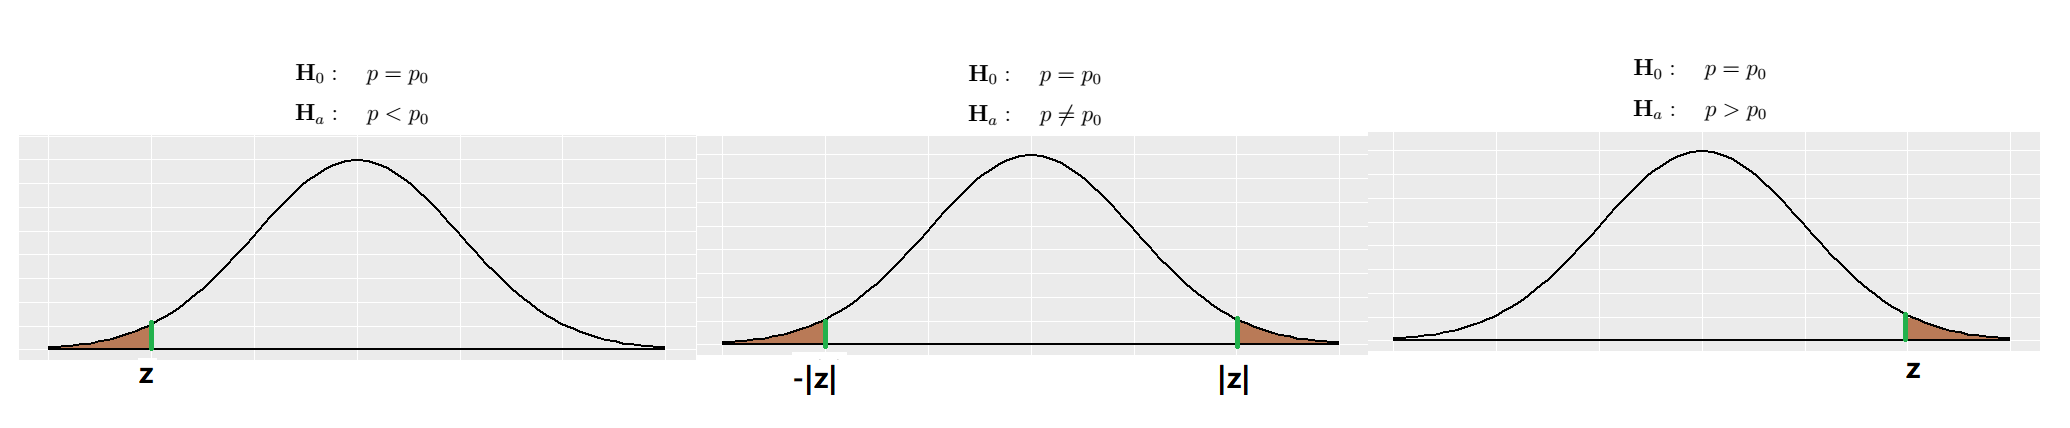
\includegraphics[scale=0.4]{TestStatisticAndPvalue}
\caption{P-value in different cases for statistic $z$}
\label{TestStatisticAndPvalue}
\end{figure}


 \item \textbf{General steps}\vspace{0.3cm}

\begin{itemize}
  \item \textbf{State correct hypotheses and set the significance level}
  \item \textbf{Identify correct test and check conditions}
  \item \textbf{Calculate P-value: shall report test statistic, degree of freedom, etc.}
  \item \textbf{Conclude}
\end{itemize}

\colorbox{babypink}{\parbox{0.9\textwidth}{
\textbf{Remark:}\vspace{0.3cm}

All the previous formulas about hypotheses test is built on the prerequisite that the sampling distribution is a normal distribution, thus the conditions to be checked is exactly the same as the corresponding confidence intervals.
}}
\newpage



\colorbox{champagne}{\parbox{0.9\textwidth}{
\item \textbf{Example}\vspace{0.3cm}

A potato chip producer and its main supplier agree that each shipment of potatoes must meet certain quality standards. If the producer determines that more than 8\% of the potatoes in the shipment have “blemishes,” the truck will be sent away to get another load of potatoes from the supplier. Otherwise, the entire truckload will be used to make potato chips.\vspace{0.3cm}

 A supervisor selects a random sample of 500 potatoes from the truck. An inspection reveals that 47 of the potatoes have blemishes. Carry out a significance test at the $\alpha = 0.05$ significance level.  What should the chi producer conclude?\vspace{0.3cm}
 
 \textbf{Solution:}\vspace{0.3cm}
 
 \begin{itemize}
    \item \textbf{Set up hypotheses}
        $$\textbf{H}_0:\quad p = 0.08$$
        $$\textbf{H}_0:\quad p > 0.08$$
        where $p$ is the percentage of potatoes in the shipment have blemishes.
      \item We will perform a one-sample z test for $p$ if conditions are met.
         \begin{itemize}
            \item \textbf{Random:} the sample is a random sample by the stem of the problem.
               \begin{itemize}
               \item \textbf{10\% condition} The sample size 500 is less than 10\% of the total truck load of potatoes
               \end{itemize}
              \item \textbf{Large counts condition:} 
              $$np = 500\cdot 0.08 = 40 \geq 10, \quad n(1-p) = 500\cdot(1-0.08) = 460\geq 10$$  
              Large counts condition is met.              
         \end{itemize}\vspace{0.3cm}
    
       
    \item \textbf{Calculate P-value}\vspace{0.3cm}
       
       The test statistic $\displaystyle{z= \frac{\reallywidehat{p}-p}{\sigma_{\reallywidehat{p}}} = (\frac{47}{500}-0.08)\Bigg/\sqrt{\frac{0.08(1-0.08)}{500}} = 1.15}$
       The P-value$\textbf{P}(z\geq 1.15)$ given by command \texttt{normalcdf(lower:1.15, upper: $\infty$, $\mu = 0$, $\sigma =1$)} is 0.1251.\vspace{0.3cm}
    \item \textbf{Conclusion}
    
    Since the P-value is 0.1251 larger than the significance level 0.05, we fail to reject the null hypotheses, and don't have convincing evidence that the percentage of potatoes in the shipment have blemishes if larger than 8\%. The producer should use the potatoes to make chips.
 \end{itemize} 
}}
\end{itemize}
    \begin{textblock}{3.6}(14.8, -10)
    \textblockcolor{dollarbill}
    When checking the \textit{large counts condition}, why do we use $np$ and $n(1-p)$ instead of $n\reallywidehat{p}$ and $n(1-\reallywidehat{p})$?
    \end{textblock}
\newpage
\colorbox{champagne}{\parbox{\textwidth}{
\textbf{Teen Drivers}\vspace{0.3cm}

 A state’s Division of Motor Vehicles (DMV) claims that 60\% of teens pass their driving test on the first attempt. An investigative reporter examines an SRS of the DMV records for 125 teens; 86 of them passed the test on their first try. Is there convincing evidence at the a = 0.05 significance level that the DMV’s claim is incorrect? 
}}
\newpage

\section{Type I error and type II error}

Let take a look at a \textit{one-sided hypotheses test} with hypotheses 
$$\textbf{H}_0: \quad p=p_0$$
$$\textbf{H}_a: \quad p<p_0$$
The significance level is $\alpha$.
The basic idea of hypotheses test is, assuming $\textbf{H}_0$ is true, if we draw a sample and the sample statistic is too far away from the parameter given by $\textbf{H}_0$ in the direction of $\textbf{H}_a$, then we reject $\textbf{H}_0$, have convincing evidence for $\textbf{H}_a$.

  \begin{figure}[H]
  \centering
  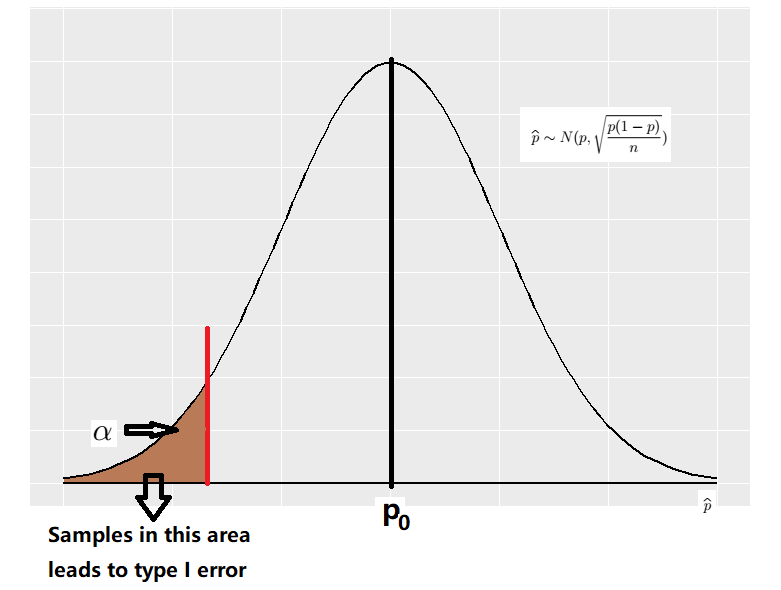
\includegraphics[scale=0.5]{TypeOneError}
  \caption{Type I error equals significance level $\alpha$}
  \label{TypeOneError}
  \end{figure}

As shown in figure\ref{TypeOneError}, if $\textbf{H}_0$ is really true,  there are still some samples in the shaded area with P-value less than significance level $\alpha$, and lead to a wrong conclusion by rejecting $\textbf{H}_0$. The probability of making this type of wrong conclusion equals significance level $\alpha$. \vspace{0.3cm}


\colorbox{babypink}{\parbox{\textwidth}{
\textbf{Type I error} is the error that we reject $\textbf{H}_0$ when  $\textbf{H}_0$ is true.\vspace{0.3cm}

The probability of making type I error equals the significance level $\alpha$.
}}

\begin{textblock}{3}(15.5, -3)
\textblockcolor{dollarbill}
Refer to the \\``potato chip'' example in section 2. State the   \textbf{type I error} and it's consequence.
\end{textblock}
\vspace{0.3cm}

 If we set $\alpha$ at a low level, such as 0.05, and we come to the conclusion that we have convincing evidence for $\textbf{H}_a$,then we are ``pretty sure'' about this conclusion, because the probability of making mistake is 0.05. This explains why we set the conclusion we are interested in as the $\textbf{H}_a$. Why?\vspace{0.3cm}

Since the probability of \textit{type I error} is totally controlled by the significance level $\alpha$, why don't we set $\alpha$ as 0, or some value extremely small? Let's take a look at the other type of error before answering this question.\vspace{0.3cm}

Consider the same one-sided hypotheses test as above
$$\textbf{H}_0: \quad p=p_0$$
$$\textbf{H}_a: \quad p<p_0$$
The P-value is calculated while assuming $\textbf{H}_0$ is correct. As show in the first sampling distribution in figure\ref{TypeTwoError}. Any sample with sample proportion $\reallywidehat{p}$ falls to the right side of the vertical line can leads to the conclusion of ``fail to reject $\textbf{H}_0$''. If the truth is $p=p_1<p_0$, then we will make a mistake, this type of mistake is called \textbf{type II error}.\vspace{0.3cm}


\colorbox{babypink}{\parbox{\textwidth}{
\textbf{Type II error} is the error of failing to reject $\textbf{H}_0$ while $\textbf{H}_0$ is not correct.
}}

\begin{figure}[H]
\centering
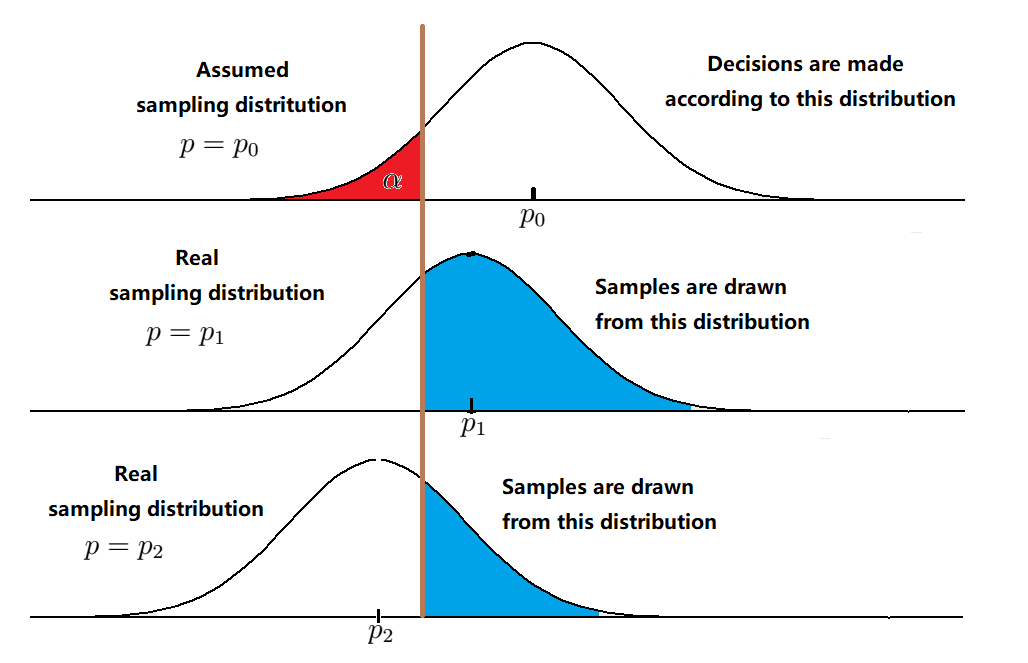
\includegraphics[scale=0.6]{TypeTwoError}
\caption{Type II error}
\label{TypeTwoError}
\end{figure}

The standard of whether to reject or fail to reject $\textbf{H}_0$ comes from the distribution while assuming $p=p_0$. However, the samples are drawn from the true sampling distribution with $p=p_1$. As shown in the second sampling distribution in figure \ref{TypeTwoError}, any sample falls in the shaded area would have P-value larger than the significance level $\alpha$, thus leads to \textit{type II error}.\vspace{0.3cm}

 The probability of making \textit{type II error} is denoted as $\beta$. $1-\beta$ is called the \textbf{power} of the test.\vspace{0.3cm}

\begin{textblock}{3.2}(-3.6, -2)
\textblockcolor{dollarbill}
Can you find out the areas that represent $\beta$ and the \textit{power} in figure \ref{TypeTwoError}?
\end{textblock}
\vspace{0.3cm}

How to increase the \textit{power} of a test?
    \begin{itemize}
       \item \textbf{Increase the significance level $\alpha$}\vspace{0.3cm}. This is indicated in figure \ref{TypeTwoError}. It means there is a trade off between the probability of type I error and the probability of type II error.
       \item \textbf{Increase the difference between the null and alternative parameter values that is important to detect.} This is shown in figure \ref{TypeTwoError}, when the true value of $p$ takes $p_1$ and $p_2$ separately.
       \item \textbf{Increase the sample size.} Suppose the true value of $p$ is $p_1$.
          \begin{equation*}
             \begin{split}
             \textbf{Power}&=\textbf{P}\Bigg(\reallywidehat{p} < p_0 + z_{\alpha}\sqrt{\frac{p_0(1-p_0)}{n}}\Bigg)\\
             &= \textbf{P}\Bigg(\frac{\reallywidehat{p}-p_1}{\sqrt{\frac{p_1(1-p_1)}{n}}} < \frac{p_0 + z_{\alpha}\sqrt{\frac{p_0(1-p_0)}{n}} - p_1}{\sqrt{\frac{p_1(1-p_1)}{n}}}\Bigg)\\    
             &= \textbf{P} \Bigg(z_{\reallywidehat{p}} < \frac{p_0-p_1}{\sqrt{p_1(1-p_1)}}\sqrt{n} + z_{\alpha}\sqrt{\frac{p_0(1-p_0)}{p_1(1-p_1)}}\Bigg)      
             \end{split}
          \end{equation*}
  where $z_{\alpha}$ is the z-score with $\textbf{P}(z<z_{\alpha}) = \alpha$
  
  \begin{textblock}{4}(-3, -4)
  \textblockcolor{dollarbill}
  Can you explain in detail the equations for the \textit{power}?
  \end{textblock}
  
  From the equation, we know that as sample size $n$ increases, the \textit{power} of the test increase. 
    \end{itemize}
\newpage
\colorbox{champagne}{\parbox{\textwidth}{
\textbf{Protect your own interest}\vspace{0.3cm}

Refer to previous example about the potatochi producer and its main supplier. Answer the following questions.
\begin{enumerate}[(a)]
    \item State the \textit{type II error} and it's consequence.
    \item If your are the potato chip producer, would you prefer a larger significance level $\alpha$ or a smaller one?
    What if you are the main supplier?
    \item According to the result of the example, what type of mistake may be made?
\end{enumerate}
}}

\newpage
\section{Two-sample z test for $p_1-p_2$}

Take a one-sided hypotheses test for example.\vspace{0.3cm}

Population 1 is with proportion $p_1$ and population size $N_1$. Population 2 is with proportion $p_2$ and population size $N_2$. Is $p_1>p_2$ ? In order to test this hypotheses, we draw an SRS with size $n_1$ from population 1, and an SRS with size $n_2$ from population 2. The sample proportions for those two samples are $\reallywidehat{p}_1$ and $\reallywidehat{p}_2$ respectively.\vspace{0.3cm}

The general steps are the same as \textit{one-sample z test for population proportion} except for a few things we should pay attention to.\vspace{0.3cm}


The hypotheses are
$$\textbf{H}_0:\quad p_1-p_2 =0$$
$$\textbf{H}_0:\quad p_1-p_2 >0$$

\begin{itemize}
\item \textbf{Large counts condition}\vspace{0.3cm}

When assuming $\textbf{H}_0$ is true, we know $p_1=p_2$, but don't know the exact value. When checking the large counts condition we check the following
$$n_1\reallywidehat{p}_1\geq 10, \quad n_1(1-\reallywidehat{p}_1)\geq 10; \qquad n_2\reallywidehat{p}_2\geq 10, \quad n_2(1-\reallywidehat{p}_2)\geq 10$$

\item \textbf{The test statistic $z$}\vspace{0.3cm}

$$\textbf{Test statistic}= \frac{\textbf{statistic}-\textbf{parameter}}{\textbf{standard deviation of the statistic}}$$

$$z=\frac{(\reallywidehat{p}_1-\reallywidehat{p}_2)-0}{\sigma_{\reallywidehat{p}_1-\reallywidehat{p}_2}}=\frac{(\reallywidehat{p}_1-\reallywidehat{p}_2)-0}{\sqrt{\frac{p_1(1-p_1)}{n_1}+\frac{p_2(1-p_2)}{n_2}}}$$

Since we don't know $p_1$ and $p_2$, we can replace them by $\reallywidehat{p}_1$ and $\reallywidehat{p}_2$. But, the test statistic $z$ is calculated when assuming $\textbf{H}_0$ is true, that is $p_1-p_2=0$. Therefore $p_1$ and $p_2$ should be replaced by the same value instead of $\reallywidehat{p}_1$ and $\reallywidehat{p}_2$ separately. We replace $p_1$ and $p_2$ by the following value.
$$\reallywidehat{p}_C= \frac{X_1+X_2}{n_1+n_2}$$
where $X_1$ and $X_2$  are the numbers of ``success'' in the two samples.
$$X_1 = n_1\reallywidehat{p}_1,\quad X_1 = n_2\reallywidehat{p}_2$$

$\reallywidehat{p}_C$ is called the \textbf{pooled(combined) sampled proportion}.\vspace{0.3cm}

The formula for test statistic $z$ is
$$z=\frac{(\reallywidehat{p}_1-\reallywidehat{p}_2)-0}{\sqrt{\frac{\reallywidehat{p}_C(1-\reallywidehat{p}_C)}{n_1}+\frac{\reallywidehat{p}_C(1-\reallywidehat{p}_C)}{n_2}}}.$$
\end{itemize}
\newpage
\colorbox{champagne}{\parbox{\textwidth}{
\textbf{Cholesterol and Hear Attacks}\vspace{0.3cm}

High levels of cholesterol in the blood are associated with higher risk of heart attacks. Will using a drug to lower blood cholesterol reduce heart attacks? The Helsinki Heart Study recruited middle-aged men with high cholesterol but no history of other serious medical problems to investigate this question. The volunteer subjects were assigned at random to one of two treatments: 2051 men took the drug gemfibrozil to reduce their cholesterol levels, and a control group of 2030 men took a placebo. During the next five years, 56 men in the gemfibrozil group and 84 men in the placebo group had heart attacks. 
\begin{enumerate}[(a)]
\item Is this difference statistically significant at the $\alpha = 0.01$ level?
\item Construct a 1\% confidence interval for the difference of the ratios of heart attacks between those who take drugs and those who take placebos.
\item Compare the above two results.
\end{enumerate}
}}
\newpage
\section{One-sample z test for $\mu$\\ One-sample t test for $\mu$}

\begin{itemize}
\item \textbf{One-sample z test for $\mu$}\vspace{0.3cm}

 A two-sided hypotheses test is: there is a population with size $N$, population mean $\mu_0$ and standard deviation $\sigma$. Now we are suspect that the population mean might be different from $\mu_0$. In order to test this suspicion, an SRS with size $n$ is drawn from the population, and the sample mean is $\bar{x}$. What is the conclusion about the suspicion?\vspace{0.3cm}
 
 We follow the sample procedure as before: set up hypotheses and significance level, identify correct test and check conditions, calculate P-value and conclude.\vspace{0.3cm}
 
 In this setting the hypotheses are
 $$\textbf{H}_0: \quad \mu = \mu_0$$
  $$\textbf{H}_a: \quad \mu \ne \mu_0$$
 
 The conditions to be checked is exactly the same as the conditions to be checked when constructing \textit{one-sample z interval for $\mu$}.
 
 The test statistic is given by 
 $$z=\frac{\bar{x}-\mu_0}{\frac{\sigma}{\sqrt{n}}}$$
 
 \item \textbf{One-sample t test for $\mu$}\vspace{0.3cm}
 
 In the above setting, if we don't know the standard deviation of the population, we have to use \textit{one-sample t test for $\mu$}. This situation is the same as constructing \textit{one-sample t interval for $\mu$}.\vspace{0.3cm}
 
Everything is the same as \textit{one-sample z test for $\mu$}, except the test statistic. 
 $$t=\frac{\bar{x}-\mu_0}{\frac{s_X}{\sqrt{n}}}, \quad df = n-1$$
 \textbf{Be sure to report the \textit{degree of freedom} in the exam.}\vspace{0.3cm}
\end{itemize}
\newpage
\colorbox{champagne}{\parbox{\textwidth}{
\textbf{Paying High Prices?}\vspace{0.3cm}

 A retailer entered into an exclusive agreement with a supplier who guaranteed to provide all products at competitive prices. The retailer eventually began to purchase supplies from other vendors who offered better prices. The original supplier filed a lawsuit claiming violation of the agreement. In defense, the retailer had an audit performed on a random sample of 25 invoices. For each audited invoice, all purchases made from other suppliers were examined and compared with those offered by the original supplier. The percent of purchases on each invoice for which an alternative supplier offered a lower price than the original supplier was recorded.21 For example, a data value of 38 means that the price would be lower with a different supplier for 38\% of the items on the invoice. A histogram and some computer output for these data are shown below. Explain why we should not carry out a one-sample t test in this setting.
 
 \begin{figure}[H]
 \centering
 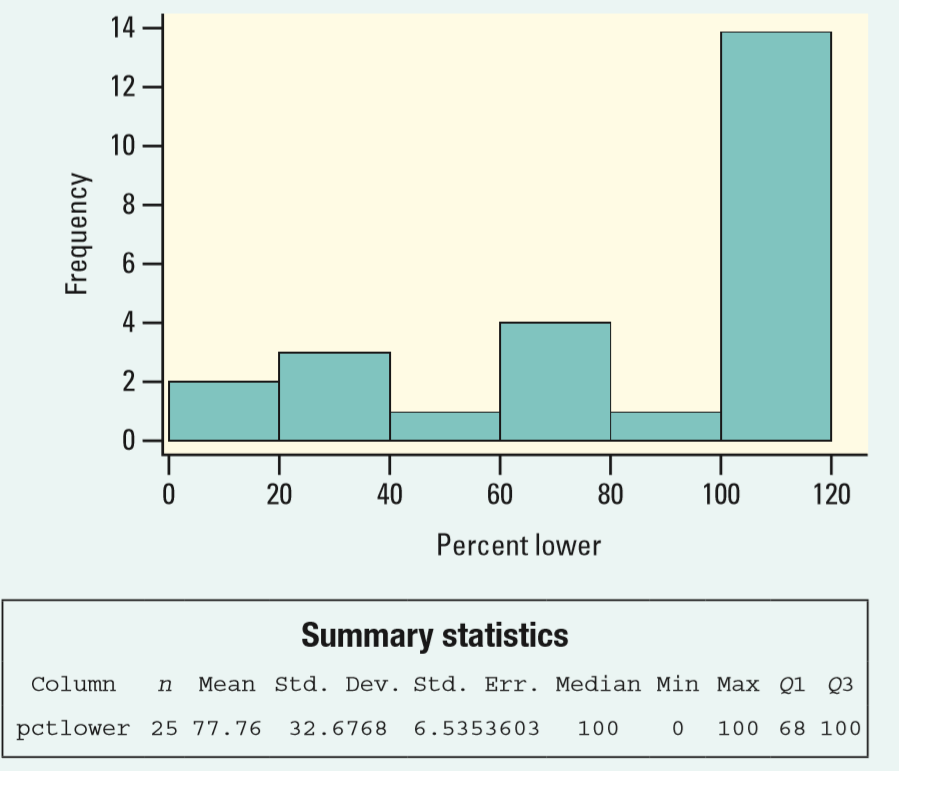
\includegraphics[scale=0.6]{ExerciseForCheckingConditionsForOneTMean}
 \label{ExerciseForCheckingConditionsForOneTMean}
 \end{figure}
}}
\newpage
\colorbox{champagne}{\parbox{\textwidth}{
\textbf{Interpreting the output}\vspace{0.3cm}

The recommended daily allowance (RDA) of calcium for women between the ages of 18 and 24 years is 1200 milligrams (mg). Researchers who were involved in a large-scale study of women’s bone health suspected that their participants had significantly lower calcium intakes than the RDA. To test this suspicion, the researchers measured the daily calcium intake of a random sample of 36 women from the study who fell in the desired age range. The Minitab output below displays the results of a significance test.\vspace{0.3cm}

    \begin{table}[H]
    \centering
       \begin{tabular}{|lcccccc|}
       \hline
       \multicolumn{7}{|c|}{\textbf{Summary statistics}}\\
       \multicolumn{7}{|l|}{\texttt{Test of mu = 1200 vs < 1200}}\\
       \texttt{Variable}& \texttt{N}& \texttt{Mean}&\texttt{StDev}&\texttt{SE Mean}&\texttt{T}&\texttt{P}\\
       \texttt{Calcium}&\texttt{36}&\texttt{856.2}&\texttt{306.7}&\texttt{51.1}&\texttt{ −6.73}&\texttt{ 0.000}\\  
       \hline   
       \end{tabular}
    \end{table}
    
    \begin{enumerate}[(a)]
       \item Do these data give convincing evidence to support the researchers’ suspicion? Justify your answer.
       \item Interpret the P-value in context.
    \end{enumerate}
}}

\newpage
\colorbox{champagne}{\parbox{\textwidth}{
\textbf{Flu Vaccine}\vspace{0.3cm}

A drug company has developed a new vaccine for preventing the flu. The company claims fewer than 5\% of the adults who use its vaccine will get the flu. To test the claim, researchers give the vaccine to a random sample of 1000 adults. Of these, 43 get the flu.
  \begin{enumerate}[(a)]
      \item Do these data provide convincing evidence to support the company’s claim?
      \item Which kind of mistake, Type I error or  Type II error, could you have made in (a)? Explain.
      \item From the company’s point of view, would a Type I error or Type II error be more serious? Why?
  \end{enumerate}
}}
\newpage
\section{Two-sample z test for $\mu_1-\mu_2$\\Two-sample t test for $\mu_1-\mu_2$}
\begin{itemize}
   \item \textbf{Two-sample z test for $\mu_1-\mu_2$}\vspace{0.3cm}
   
   A one-sided hypotheses test might be setted as this.  There are population 1 and population 2 with the standard deviation $\sigma_1$ and $\sigma_2$ respectively, and the alleged difference of the population means is $\mu_1-\mu_2=D$. We suspect the difference might be smaller. To test our suspicion, an SRS is drawn from population 1, with sample size $n_1$ , sample mean $\bar{x}_1$ and sample standard deviation $s_1$, the other SRS is drawn from population 2 with sample size $n_2$ , sample mean $\bar{x}_2$ and sample standard deviation $s_2$. What can we conclude from this.\vspace{0.3cm}
   
   The hypotheses are
   $$\textbf{H}_0:\quad \mu_1-\mu_2 = D$$
   $$\textbf{H}_a:\quad \mu_1-\mu_2 < D$$
   
   The conditions to be checked is exactly the same as the conditions checked when constructing two-sample z interval for $\mu_1-\mu_2$.\vspace{0.3cm}
   
   The test statistic z is given by 
   $$z=\frac{\bar{x}_1- \bar{x}_2-D}{\sigma_{\bar{x}_1- \bar{x}_2}} = \frac{\bar{x}_1- \bar{x}_2-D}{\sqrt{\frac{\sigma_1^2}{n_1} + \frac{\sigma_2^2}{n_2}}}$$
   
 \item \textbf{Two-sample t test for $\mu_1-\mu_2$} \vspace{0.3cm}
 
  The setting is the same as above, except that we don't know the standard deviations of the populations \vspace{0.3cm}
  
  The conditions to be checked is exactly the same as the conditions checked in constructing the two-sample t interval for $\mu_1-\mu_2$\vspace{0.3cm}
  
  The test statistic if given by 
   $$t=\frac{\bar{x}_1- \bar{x}_2-D}{\textbf{SE}_{\bar{x}_1- \bar{x}_2}} = \frac{\bar{x}_1- \bar{x}_2-D}{\sqrt{\frac{s_1^2}{n_1} + \frac{s_2^2}{n_2}}}$$
   
   The degree of freedom of $t$ are given by either a conservative method, $min(n_1-1, n_2-1)$, or by \textit{technology}. This is the same as when we construct the two-sample t interval for $\mu_1-\mu_2$.\vspace{0.3cm}
   
   \colorbox{babypink}{\parbox{0.9\textwidth}{
   Most of the time, we just report the degree of freedom given by the calculator.
   }}
\end{itemize}





\newpage
 \colorbox{champagne}{\parbox{\textwidth}{
 \textbf{Calcium and Blood Pressure}\vspace{0.3cm}
 
 Does increasing the amount of calcium in our diet reduce blood pressure? Examination of a large sample of people revealed a relationship between calcium intake and blood pressure. The relationship was strongest for black men. Such observational studies do not establish causation. Researchers therefore designed a randomized comparative experiment.\vspace{0.3cm}
 
 The subjects were 21 healthy black men who volunteered to take part in the experiment. They were randomly assigned to two groups: 10 of the men received a calcium supplement for 12 weeks, while the control group of 11 men received a placebo pill that looked identical. The experiment was doubleblind. The response variable is the decrease in systolic (top number) blood pressure for a subject after 12 weeks, in millimeters of mercury. An increase appears as a negative number. Here are the data:
 \begin{table}[H]
 \centering
 \begin{tabular}{lcccc ccccc cc}
 \hline
 \textbf{Group 1 (calcium):}&7 &−4 &18 &17 &−3& −5 &1 &10 & 11& −2&\\
 \textbf{Group 2 (placebo):}&−1 &12 &−1 &−3 & 3 &−5& 5  &2& −11& −1 &−3\\
 \hline
 \end{tabular}
 \end{table} 
 }}
\newpage
\colorbox{babypink}{\parbox{\textwidth}{
In the matched pairs design, it looks like we have got two set of data, and we should perform a two-sample hypotheses test or construct a two-sample confidence interval. In reality, we only have one set of date, which is the difference within each pair.
}}
\vspace{0.3cm}

\colorbox{champagne}{\parbox{\textwidth}{
Refer to the exercise ``\textbf{Nitrogen in tires \textemdash a lot of hot air} '' in the chapter of ``\textbf{Designing studies}''. Answer the following questions.
   \begin{enumerate}[(a)]
      \item Perform a hypotheses test under the significance level $\alpha = 0.05$ to test the claim that filling automobile tires with nitrogen reduces pressure loss.
      \item Construct a 95\% confidence interval for the  difference of the mean pressure loss between tires filled with air and tires filled with nitrogen.
   \end{enumerate}
}}
\newpage
\textbf{Investigation problems with simulated sampling distribution}\vspace{0.6cm}

  \colorbox{champagne}{\parbox{\textwidth}{
  \textbf{The accuracy of EKG}\vspace{0.3cm}
  
  An exercise electrocardiogram (EKG) checks for changes in your heart during exercise and is useful in diagnosing coronary artery disease. An EKG has fewer potential side effects but is much less precise than thallium tomography. In one EKG study, 500 volunteers with known coronary artery disease and 500 volunteers with healthy arteries underwent EKG checks. The physicians administering and evaluating the tests did not know the physical condition of any volunteer. The following table gives the numbers of volunteers whom the physicians evaluated as  ``positive'' for coronary disease. 
  
        \begin{table}[H]
       \centering
        \begin{tabular}{lcr}
        \hline
        &\multicolumn{2}{c}{\textbf{Test for coronary disease}}\\
        \cline{2-3}\\
        &\textbf{Positive}&\textbf{Negative}\\
        Healthy volunteers&$100$&$400$\\
    Volunteers with disease& $305$ &  $195$\\
    \hline
        \end{tabular}
     \end{table}
  \begin{enumerate}[(a)]
      \item \textit{Sensitivity} is defined as the probability of a positive test given that the subject has disease. What was the sensitivity of this study?
      \item \textit{Specificity} is defined as the probability of a negative test given that the subject is healthy. What was the specificity of this study?
      \item A valuable tool for assessing the accuracy of such studies is the \textit{positive diagnostic likelihood ratio} ($\text{LR}^+$) which gives the ratio of the probability a positive test result will be observed in a diseased person compared to the probability that the same result will be observed in a healthy person.
      $$\text{LR}^+ = \frac{\text{sensitivity}}{1-\text{specificity}}$$
      
      What was $\text{LR}^+$ in this study, and explain why the larger the value of $\text{LR}^+$, the more useful the test.
      \item  Suppose in one such sample study, $\text{LR}^+ = 4.7$. To determine whether or not this is sufficient evidence that the population $\text{LR}^+$ is below the desired value of 5.0, 100 samples from a population with a known $\text{LR}^+$ of 5.0 are generated, and the resulting simulated values of $\text{LR}^+$ are shown in the dotplot:
      \begin{figure}[H]
      \centering
      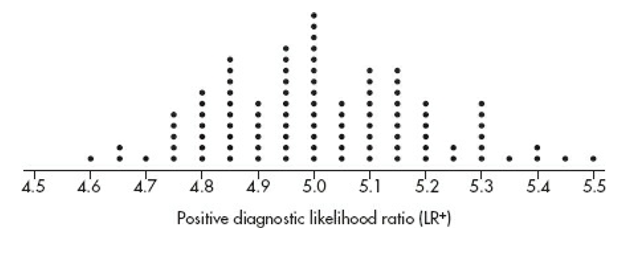
\includegraphics[scale=0.6]{InvestigationHT}
      \end{figure}
      
      
   Based on this dotplot and the sample $\text{LR}^+ = 4.7$, is there evidence that the population $\text{LR}^+$ is below the desired value of 5.0? Explain.
  \end{enumerate}  
  }}

\end{document}